% ==========================================================
% sound_tamil.tex — ஒலி (Sound)
% TNSCERT 8ஆம் வகுப்பு அறிவியல்
% தமிழாக்கம்: TNSCERT Workshop (Nov 2025 & Mar 2026)
% அசல் ஆசிரியர்: Disha Kuzhively
%
% Compile: xelatex sound_tamil.tex
% Font: Noto Sans Tamil (install before compiling)
% ==========================================================

\documentclass[12pt,a4paper]{tufte-handout}

% ---- Tamil & Unicode support ----
\usepackage{fontspec}
\setmainfont[
  Script=Tamil,
  BoldFont={Noto Sans Tamil Bold},
  ItalicFont={Noto Sans Tamil},
]{Noto Sans Tamil}
\newfontfamily\englishfont{Latin Modern Roman}

\usepackage{polyglossia}
\setmainlanguage{tamil}
\setotherlanguage{english}

% ---- Packages ----
\usepackage{graphicx}
\usepackage{amsmath}
\usepackage{booktabs}
\usepackage{multicol}
\usepackage{xcolor}
\usepackage{tcolorbox}
\usepackage{hyperref}
\usepackage{enumitem}
\usepackage{geometry}

% ---- Graphics path ----
\graphicspath{{graphics/}}

% ---- Colors ----
\definecolor{activitycolor}{RGB}{197,90,17}
\definecolor{conceptcolor}{RGB}{27,107,138}
\definecolor{teachercolor}{RGB}{100,100,100}
\definecolor{greenbox}{RGB}{55,86,35}

% ---- tcolorbox styles ----
\tcbuselibrary{skins,breakable}

\tcbset{
  activitybox/.style={
    enhanced, breakable,
    colback=orange!10,
    colframe=activitycolor,
    leftrule=4pt,
    title style={colback=activitycolor},
    fonttitle=\bfseries,
    before upper=\setlength{\parskip}{4pt},
  },
  conceptbox/.style={
    enhanced, breakable,
    colback=blue!8,
    colframe=conceptcolor,
    leftrule=4pt,
    before upper=\setlength{\parskip}{4pt},
  },
  teacherbox/.style={
    enhanced, breakable,
    colback=gray!10,
    colframe=teachercolor,
    leftrule=4pt,
    fonttitle=\bfseries,
    title={\small ஆசிரியர் குறிப்பு},
    title style={colback=teachercolor!70},
  },
  observebox/.style={
    enhanced, breakable,
    colback=blue!5,
    colframe=conceptcolor,
    leftrule=4pt,
    fonttitle=\bfseries,
    title={\small 👁 உற்று நோக்குக},
    title style={colback=conceptcolor},
  },
  discussbox/.style={
    enhanced, breakable,
    colback=blue!5,
    colframe=conceptcolor!70,
    leftrule=4pt,
    fonttitle=\bfseries,
    title={\small 💬 கலந்துரையாடல்},
    title style={colback=conceptcolor!70},
  },
  didyouknowbox/.style={
    enhanced, breakable,
    colback=green!8,
    colframe=greenbox,
    leftrule=4pt,
    fonttitle=\bfseries,
    title={💡 உங்களுக்குத் தெரியுமா?},
    title style={colback=greenbox},
  },
}

% ---- Document metadata ----
\title{ஒலி\\[0.3em]\large எட்டாம் வகுப்பு அறிவியல் --- TNSCERT}
\author{Disha Kuzhively \\ \small தமிழாக்கம்: TNSCERT 2025--2026}
\date{}

% ==========================================================
\begin{document}
\maketitle

\begin{tcolorbox}[enhanced, colback=gray!5, colframe=gray!50, fontupper=\small]
இக்கட்டுரையானது 13-11-2025 முதல் 15-11-2025 வரையிலும், மற்றும் 09-03-2026 முதல்
10-03-2026 வரையிலும் சென்னையில் உள்ள ஆஷா நிவாஸில் நடைபெற்ற தமிழ்நாடு கலைத்திட்ட
வடிவமைப்பு (TNCF) பயிலரங்கின் போது, TNSCERT 8ஆம் வகுப்பு ஒலி பாடத்துக்கான வரைவாகப்
பயன்படும் வகையில் ஆசிரியரால் உருவாக்கப்பட்டுள்ளது. ஒவ்வொரு பக்கத்தின் வலதுபுற ஓரத்திலும்
ஆசிரியர்களுக்கான குறிப்புகளும் வழிகாட்டுதல்களும் இடம்பெற்றுள்ளன.
\end{tcolorbox}

\bigskip

பள்ளி மணி ஒலிப்பது, மழைத்துளிகள் தரையில் விழுவது, நாய் குரைப்பது அல்லது தொலைபேசி
ஒலிப்பது என அன்றாடம் நம்மைச் சுற்றி பல்வேறு ஒலிகளை நாம் கேட்கிறோம்.

ஆனால், இவ்வொலிகள் எவ்வாறு உருவாகின்றன? எவ்வாறு ஒரிடத்திலிருந்து மற்றொரு
இடத்திற்குப் பரவுகின்றன? ஏன் வெவ்வேறு ஒலிகள் வெவ்வேறு பண்புகளைக்
கொண்டிருக்கின்றன? இப்பாடப் பகுதியில், ஒலி எவ்வாறு உருவாகிறது, அது எவ்வாறு
பரவுகிறது என்பதைப் பற்றி நாம் விரிவாகக் காண்போம்.

\marginnote{
\begin{tcolorbox}[teacherbox]
\small
`பயணிக்கிறது' என்ற வார்த்தைக்குப் பதிலாக `பரவுகிறது' என்ற வார்த்தை
பயன்படுத்தப்படுகிறது. மாணவர்கள் அறிவியல் ரீதியாக துல்லியமான மனச்
சித்திரத்தை உருவாக்கிக் கொள்வதற்காகவே இத்தகைய வார்த்தைகள்
கவனமாகத் தேர்ந்தெடுக்கப்பட்டுள்ளன.
\end{tcolorbox}
}

நீங்கள் அன்றாடம் கேட்டுப் பழகிய ஒலிகளை பட்டியலிடுங்கள்.

% ==========================================================
\section{ஒலி எவ்வாறு உருவாகிறது?}
% ==========================================================

\subsection*{செயல்பாடு 1: அதிர்வுறும் அளவுகோல்}

\begin{tcolorbox}[activitybox, title=தேவையான பொருட்கள்]
\begin{itemize}[noitemsep]
  \item அளவுகோலுடன் கூடிய வடிவியல் பெட்டி
  \item இரப்பர் வளையங்கள்
  \item காகிதத் தாள்கள்
  \item கத்தரிக்கோல்
\end{itemize}
\end{tcolorbox}

\begin{figure}[h]
\centering
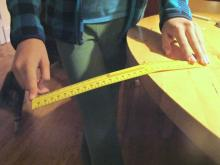
\includegraphics{scale-down}
\hspace{1em}
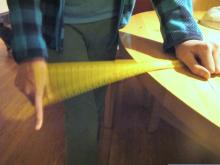
\includegraphics{scale-vibrate}
\caption{படி 1: அளவுகோலின் தடையற்ற முனையை கீழ்நோக்கி அழுத்தவும் (இடது).
         படி 2: அழுத்தப்பட்ட முனையை விடுவிக்கவும் (வலது).}
\end{figure}

அளவுகோலினை அதன் ஒரு பகுதி மேசையின் விளிம்பிற்கு வெளியே நீட்டிக்கொண்டிருக்குமாறு
மேசையில் பொருத்தவும். வெளியே நீட்டிக்கொண்டிருக்கும் அதன் தடையற்ற நுனியை
கீழ்நோக்கி அழுத்திப் பின் விடுவிக்கவும்.

\begin{tcolorbox}[observebox]
உங்களால் ஒலியினை கேட்க முடிகிறதா? அளவுகோல் வேகமாக மேலேயும் கீழேயும் நகர்வதை
உங்களால் பார்க்க முடிகிறதா? அளவுகோல் எவ்வகையான இயக்கத்தை மேற்கொள்கிறது?
\end{tcolorbox}

\subsection*{செயல்பாடு 2: இசைக்கும் வடிவியல் பெட்டி}

உங்களது வடிவியல் பெட்டியில் உள்ள பொருட்களை எடுத்துவிட்டு, பெட்டியைக் காலியாக்குங்கள்.
ஒரு இரப்பர் வளையத்தை அந்தக் காலியான பெட்டியைச் சுற்றி இறுக்கமாகப் பொருத்துங்கள்.
இப்போது அந்த இரப்பர் வளையத்தை விரலால் சுண்டியோ அல்லது இழுத்தோ விடுங்கள்.

\begin{tcolorbox}[observebox]
உங்களுக்கு ஏதேனும் ஒலி கேட்கிறதா? இவ்வமைப்பில் எப்பகுதி நகர்கிறது?
\end{tcolorbox}

\subsection*{செயல்பாடு 3: காகித விசில்}

படத்தில் காட்டியவாறு ஒரு காகித விசிலை நீங்களே உருவாக்கி, அதன் திறந்த முனையின்
வழியாகக் காற்றை உள்ளே இழுக்கவும்.

\begin{enumerate}[label=படி \arabic*:, leftmargin=*]
  \item ஒரு காகிதத் துண்டை எடுத்துக் கொள்ளவும்.
  \item புள்ளியிடப்பட்ட கோட்டின் வழியே வெட்டவும்.
  \item AB-இன் மீது ஒரு பென்சிலை வைத்து, காகிதத்தை உருளை வடிவத்தில் சுருட்டவும்.
  \item பென்சிலை வெளியே எடுக்கவும். உருளையின் ஒரு பக்கத்தை மூடும் வகையில்
        காகித மடிப்பை மடிக்கவும்.
\end{enumerate}

\subsection*{கூடுதல் செயல்பாடு: இசைக்கவை}

\begin{marginfigure}
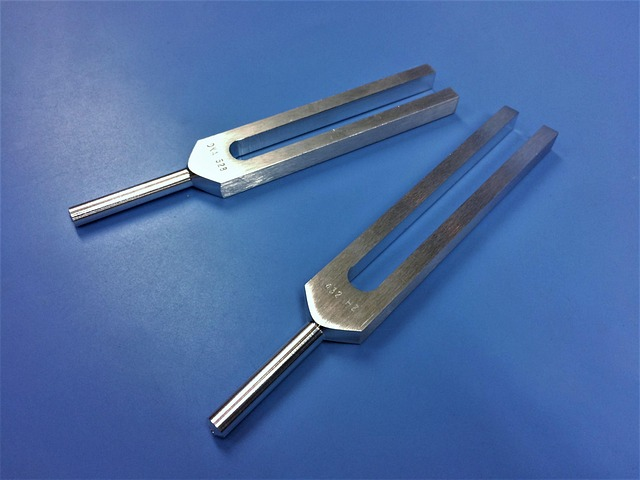
\includegraphics{tuning-fork}
\caption{இசைக்கவை}
\end{marginfigure}

இசைக்கவை கிடைக்குமானால் இச்செயல்பாட்டை மேற்கொள்ளலாம்.

இசைக்கவையின் ஒரு புயத்தை இரப்பர் சுத்தியலால் மெதுவாகத் தட்டி அதனை அதிர்வுறச் செய்யவும்.
அதிர்வடையும் அந்த இசைக்கவையை உங்கள் காதிற்கு அருகில் கொண்டு வாருங்கள். உங்களால்
ஒலியைக் கேட்க முடிகிறதா? அதிர்வுறும் புயங்களை ஒரு கிண்ணத்தில் உள்ள நீரின்
மேற்பரப்பில் மெதுவாகத் தொடுமாறு வையுங்கள். நீரின் பரப்பில் சிற்றலைகள்
உருவாவதை உங்களால் காண முடிகிறதா?

\begin{tcolorbox}[discussbox]
மேற்கண்ட ஒவ்வொரு நிகழ்விலும், பொருளின் ஏதேனும் ஒரு பகுதி வேகமாக முன்னும் பின்னுமாக
நகர்கிறது. இவ்வகையான இயக்கமே \textbf{அதிர்வுறும் இயக்கம்} என அழைக்கப்படுகிறது.
\end{tcolorbox}

\begin{tcolorbox}[conceptbox]
\textbf{முக்கிய கருத்து:} பொருட்கள் \textbf{அதிர்வடையும்} போது ஒலி உருவாகிறது.

ஒரு பொருளின் அதிர்வடையும் பகுதியானது, அதன் சுற்றியுள்ள காற்று அல்லது நீர்
போன்றவற்றை அதிர்வடையச் செய்து சிற்றலைகளை உருவாக்குகிறது. இந்த அதிர்வலைகளே
ஒலியாகப் பரவி நம்மை வந்தடைகின்றன.
\end{tcolorbox}

\bigskip

\noindent\textbf{அட்டவணை 1: உற்றுநோக்கல் அட்டவணை}

அட்டவணையில் கொடுக்கப்பட்டுள்ளவாறு, ஒலியை உருவாக்கும் பொருட்களையும்,
அப்பொருட்களில் அதிர்வடையும் பகுதிகளையும் பட்டியலிட்டு ஓர் அட்டவணை உருவாக்கவும்.

\begin{table}[h]
\centering
\begin{tabular}{|c|p{4cm}|p{4cm}|}
\hline
\textbf{வ. எண்} & \textbf{ஒலியை உருவாக்கும் பொருள்} & \textbf{அதிர்வடையும் பகுதி} \\
\hline
1 & அதிர்வடையும் அளவுகோல் & அளவுகோலின் நுனிப்பகுதி \\
\hline
2 & இசைக்கும் வடிவியல் பெட்டி & \dotfill \\
\hline
3 & \dotfill & \dotfill \\
\hline
4 & \dotfill & \dotfill \\
\hline
5 & \dotfill & \dotfill \\
\hline
\end{tabular}
\end{table}

\begin{tcolorbox}[didyouknowbox]
பல குவார்ட்ஸ் சுவர்க் கடிகாரங்கள் மற்றும் கைக்கடிகாரங்களில் நேரத்தைத் துல்லியமாகக்
கணக்கிட ஒரு சிறிய குவார்ட்ஸ் படிகம் பயன்படுத்தப்படுகிறது. இப்படிகமானது ஒரு சிறிய
இசைக்கவையைப் போன்ற வடிவத்தைக் கொண்டுள்ளது.
\end{tcolorbox}

% ==========================================================
\section{ஒலி எவ்வாறு பரவுகிறது?}
% ==========================================================

\subsection*{செயல்பாடு 4: வெற்றிடத்தில் ஒலி}

\begin{tcolorbox}[activitybox, title=தேவையான பொருட்கள்]
\begin{itemize}[noitemsep]
  \item அலைபேசி
  \item காற்றுப்புகாத கலன்
\end{itemize}
\end{tcolorbox}

அலைபேசியில் இசையை ஒலிக்கச் செய்து, அதனை ஒரு காற்றுப்புகாத கலனுக்குள் வைக்கவும்.
கலனின் மூடியை நன்கு இறுக்கமாக மூடவும்.

\begin{tcolorbox}[observebox]
அலைபேசியில் இருந்து வெளிவரும் ஒலியானது இப்போது கேட்கிறதா?
\end{tcolorbox}

\begin{tcolorbox}[discussbox]
ஒலியானது காற்றின் வழியே பரவி நமது காதுகளை வந்தடைகிறது. \textbf{வெற்றிடத்தின் வழியே
ஒலியால் பரவ முடியாது} --- அதாவது வெற்றிடத்தில் ஒலி பரவாது.
\end{tcolorbox}

\subsection*{செயல்பாடு 5: மரம் அல்லது உலோகத்தின் வழியே ஒலியைக் கேட்டல்}

உங்களது காதை மேசையின் மீது வைக்கவும். உங்களுடன் அமர்ந்துள்ள மாணவரை உங்கள்
காதிலிருந்து சிறிது தொலைவில், மேசையின் மீது ஒரு பென்சிலால் மெதுவாகத் தட்டுமாறு கூறவும்.

\begin{tcolorbox}[observebox]
மேசையின் வழியே கேட்கும் ஒலியானது பொதுவாக அதிக சத்தத்துடனோ அல்லது தெளிவாகவோ கேட்கும்.
\end{tcolorbox}

\begin{marginfigure}
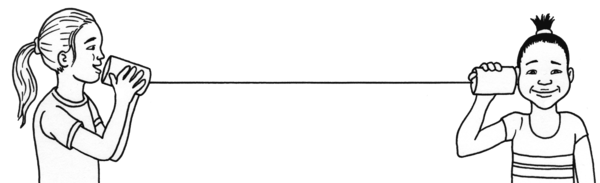
\includegraphics{stringtelephone}
\caption{நூல் தொலைபேசி --- திடப்பொருள் வழியாக ஒலி பரவல்}
\end{marginfigure}

\begin{tcolorbox}[conceptbox]
ஒலி பரவுவதற்கு ஒரு \textbf{ஊடகம்} (காற்று, நீர் அல்லது திடப்பொருள் போன்றவை) தேவைப்படுகிறது.
எந்த பொருளின் வழியே ஒலி பரவுகிறதோ, அந்த பொருள் `ஊடகம்' என அழைக்கப்படுகிறது.
\end{tcolorbox}

\subsection*{செயல்பாடு 6: ஒலியுடன் காற்றும் சேர்ந்து பயணிக்கிறதா?}

\begin{tcolorbox}[activitybox, title=தேவையான பொருட்கள்]
\begin{itemize}[noitemsep]
  \item மெல்லிய காகிதத்தாள் அல்லது ஒரு மெழுகுவர்த்தி
  \item ஒலியை உருவாக்கும் பொருள் (உதாரணமாக ஒரு மணி)
\end{itemize}
\end{tcolorbox}

மெழுகுவர்த்தியை ஒலியை உருவாக்கும் மூலத்திலிருந்து சுமார் 20--30 செ.மீ தொலைவில்
வைக்கவும். இப்போது ஒலியை எழுப்பவும்.

\begin{tcolorbox}[observebox]
மெழுகுவர்த்தியின் சுடரை அல்லது காகிதத் தாளை உன்னிப்பாகக் கவனிக்கவும்.
பொதுவாக அது அவ்வளவாக நகராது, அல்லது மிகச் சிறிதளவே அசையும்.
\end{tcolorbox}

\begin{tcolorbox}[discussbox]
ஒலி பரவும்போது, காற்றில் உள்ள துகள்கள் ஓரிடத்திலேயே முன்னும் பின்னுமாக அதிர்வடைகின்றன.
ஒவ்வொரு துகளும் தனக்கு அடுத்துள்ள துகளைத் தள்ளி, அந்த அதிர்வை அடுத்தடுத்துக் கடத்துகின்றன.
\textbf{அதிர்வுகள்தான்} ஊடகத்தின் வழியாகப் பரவுகின்றனவே தவிர, துகள்கள் ஒரிடத்திலிருந்து
மற்றொரு இடத்திற்கு நகர்வதில்லை.
\end{tcolorbox}

% ==========================================================
\section{ஒலி அலைகள்}
% ==========================================================

பொருள்கள் அதிர்வடையும்போது ஒலி உருவாகிறது என்பதை நாம் அறிந்துக் கொண்டோம்.
இந்த அதிர்வுகள் அதனைச் சுற்றியுள்ள காற்றை அதிர்வடையச் செய்கின்றன. ஒவ்வொரு
காற்றுத் துகளும் தனக்கு அடுத்துள்ள துகளைத் தள்ளி, அந்த அதிர்வைத்
தொடர்ச்சியாகக் கடத்துகின்றன.

\subsection{இறுக்கங்களும் தளர்ச்சிகளும்}

ஒலி காற்று வழியாகப் பரவும்போது, காற்றுத் துகள்கள் தத்தமது இடத்திலிருந்து முன்னும்
பின்னுமாக நகர்கின்றன.

\begin{tcolorbox}[conceptbox]
\begin{description}
  \item[\textbf{இறுக்கங்கள்}] காற்றுத் துகள்கள் மிக நெருக்கமாக அமைந்துள்ள பகுதிகள்.
  \item[\textbf{தளர்ச்சிகள்}] காற்றுத் துகள்கள் இடைவெளி விட்டுத் தளர்வாக அமைந்துள்ள பகுதிகள்.
\end{description}
ஓர் ஒலி அலையானது காற்று வழியாகப் பரவும்போது, இந்த இறுக்கங்களும் தளர்ச்சிகளும்
காற்று வழியே முன்னோக்கி நகர்கின்றன.
\end{tcolorbox}

\subsection*{கூடுதல் செயல்பாடு: சுருள்வில்}

\begin{marginfigure}
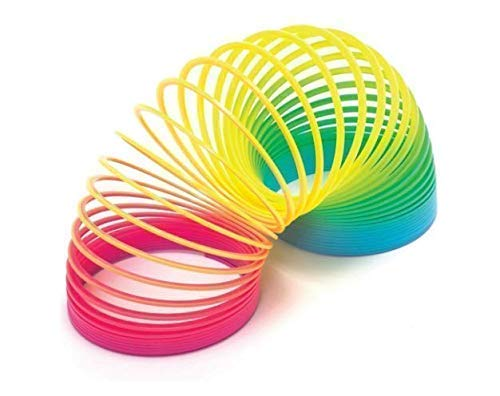
\includegraphics{slinky}
\caption{சுருள்வில் --- நெட்டலைகளை நிரூபித்தல்}
\end{marginfigure}

ஒரு `சுருள்வில்' அல்லது நீண்ட ஸ்பிரிங் ஒன்றை எடுத்துக் கொள்ளவும். அதன் ஒரு முனையை
உங்கள் நண்பரைப் பிடித்துக் கொள்ளச் சொல்லி, மறுமுனையை நீங்கள் பிடித்துக் கொள்ளவும்.
உங்கள் நண்பரை நோக்கிச் சுருள்வில்லை ஒருமுறை வேகமாகத் தள்ளவும்.

\begin{tcolorbox}[observebox]
சுருள்வில்லை அதன் நீளவாக்கிலேயே முன்னும் பின்னுமாகத் தள்ளி இழுக்கும்போது என்ன நடக்கிறது?
சுருள்வில்லின் மையத்தில் ஒரு சிறிய ரிப்பனைக் கட்டவும். அந்த ரிப்பன் எந்தத் திசையில் நகர்கிறது?
\end{tcolorbox}

\begin{tcolorbox}[conceptbox]
ஒலி அலைகளும் இவ்வாறே பரவுகின்றன. இவை \textbf{நெட்டலைகள்} என்று அழைக்கப்படுகின்றன.
திண்மம், திரவம் மற்றும் வாயுக்களின் வழியாக ஒலி நெட்டலைகளாக பரவுகிறது.
\end{tcolorbox}

% ==========================================================
\section{ஒலி எவ்வளவு வேகத்தில் பரவுகிறது?}
% ==========================================================

ஒலி உருவான உடனே அதை நாம் கேட்டுவிடுகிறோமா? மின்னல் மற்றும் இடியின் போது என்ன
நடக்கிறது என்று சிந்தித்துப் பாருங்கள்.

\begin{tcolorbox}[observebox]
நீங்கள் மின்னலை பார்ப்பதும், இடியை கேட்பதும் ஒரே நேரத்தில் நிகழ்கிறதா?
அல்லது ஒன்றன் பின் ஒன்றாக நிகழ்கிறதா? எதை முதலில் கவனிக்கிறீர்கள்?
\end{tcolorbox}

\begin{marginfigure}
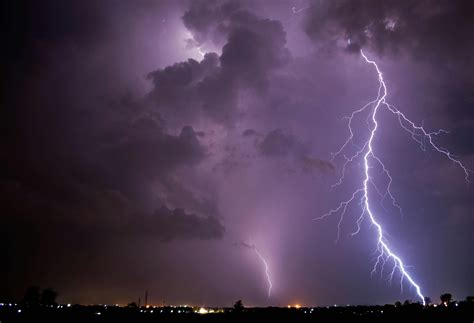
\includegraphics{thunder}
\caption{மின்னல் மற்றும் இடி --- ஒலி மற்றும் ஒளியின் வேக வேறுபாடு}
\end{marginfigure}

பொதுவாக, நாம் மின்னலை முதலில் காண்கிறோம், இடிச் சத்தத்தைச் சற்று நேரம் கழித்தே கேட்கிறோம்.

\begin{tcolorbox}[conceptbox]
\textbf{ஒலியின் வேகம்:} காற்றில், ஒலி சுமார் \textbf{340 மீட்டர்/விநாடி} (அறை வெப்பநிலையில்)
என்ற வேகத்தில் பரவுகிறது.

ஒலியின் வேகம் அது பரவும் \textbf{ஊடகத்தைப் பொறுத்தது}:
\begin{itemize}[noitemsep]
  \item திண்மங்களில் --- மிக வேகமாகப் பரவும்
  \item திரவங்களில் --- அதைவிடக் குறைவாகப் பரவும்
  \item வாயுக்களில் --- மிக மெதுவாகப் பரவும்
\end{itemize}
\end{tcolorbox}

\subsection{அதிர்வெண் மற்றும் சுருதி}

ஒரு மேசையின் விளிம்பில் ஒரு அளவுகோலை, அதன் ஒரு பகுதி வெளியே நீட்டிக்கொண்டிருக்கும்படி
வைக்கவும். வெளியே நீட்டிக்கொண்டிருக்கும் நீளத்தை மாற்றும்போது, அதன் ஒலியும் அதிர்வு
வேகமும் எவ்வாறு மாறுகின்றன என்று கவனிக்கவும்.

\begin{tcolorbox}[conceptbox]
\begin{description}
  \item[\textbf{அதிர்வெண் (Frequency, $\nu$)}] ஒரு விநாடியில் ஏற்படும் அதிர்வுகளின் எண்ணிக்கை.
        அலகு: \textbf{ஹெர்ட்ஸ் (Hz)}.
  \item[\textbf{சுருதி (Pitch)}] அதிக அதிர்வெண் $\Rightarrow$ உயர்ந்த சுருதி;
        குறைந்த அதிர்வெண் $\Rightarrow$ தாழ்ந்த சுருதி.
  \item[\textbf{வீச்சு (Amplitude)}] அதிர்வின் அளவு. அதிக வீச்சு $\Rightarrow$ அதிக உரப்பு.
\end{description}
\end{tcolorbox}

\noindent\textbf{உதாரணம்:} ஒரு மேளத்தை ஒரு விநாடியில் 10 முறை தட்டினால்,
அதிர்வெண் = \textbf{10 Hz}.

% ==========================================================
\section{அலைகளின் பண்புகள் மற்றும் அலைநீளம்}
% ==========================================================

\subsection*{செயல்பாடு: சுருள்வில் (அலைநீளம்)}

இதே சுருள்வில் செயல்பாட்டை மீண்டும் செய்யுங்கள், ஆனால் இம்முறை மிக வேகமாக
நெருக்கங்களை உருவாக்குங்கள்.

\begin{tcolorbox}[observebox]
இறுக்கங்கள் ஒன்றுக்கொன்று மிக அருகில் வருகின்றன --- இதனால் அலைநீளம் குறைகிறது.
\end{tcolorbox}

\begin{tcolorbox}[conceptbox]
அருகருகே உள்ள இரண்டு இறுக்கங்களுக்கிடைப்பட்ட தூரம் \textbf{அலைநீளம்} எனப்படும்.
அலகு: \textbf{மீட்டர் (m)}.

\begin{center}
\Large $v = \nu \times \lambda$
\end{center}
\begin{center}
\small (வேகம் = அதிர்வெண் $\times$ அலைநீளம்)
\end{center}
\end{tcolorbox}

\subsection{எதிரொலி}

ஒலி ஒரு குறிப்பிட்ட வேகத்தில் பரவுகிறது என்பதை நாம் அறிவோம். ஒளியைப் போலவே ஒலியும்
பரப்பிலிருந்து எதிரொலிக்கக் கூடியது. பிரதிபலிக்கப்பட்ட ஒலி, ஒரு குறுகிய கால
இடைவெளிக்குப் பிறகு நமது காதுகளை வந்தடையும்போது \textbf{எதிரொலி} கேட்கிறது.

\subsection{ஒலி மாசுபாடு}

போக்குவரத்து நெரிசலால் ஏற்படும் சத்தம், ஒலிபெருக்கிகள் மற்றும் தொழிற்சாலைகளின்
இரைச்சல் ஆகியவை ஒலி மாசுபாட்டிற்கு முக்கியக் காரணங்களாகும். நகரங்களில் ஒலி
மாசுபாட்டை நாம் எவ்வாறு குறைக்கலாம்?

% ==========================================================
\section{மனித காது மற்றும் செவிப்புலன்}
% ==========================================================

\begin{marginfigure}
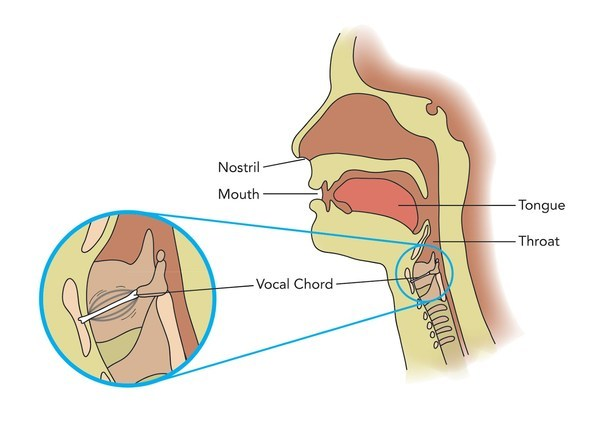
\includegraphics[width=\marginparwidth]{vocalcord}
\caption{மனித குரல்வளை}
\end{marginfigure}

மிகவும் உரத்த ஒலிகள் நமது உள் காதினைப் பாதிப்பதோடு, செவித்திறன் இழப்பிற்கும்
வழிவகுக்கும். சிலருக்குப் பிறப்பிலிருந்தே கேட்கும் திறனைப் பாதிக்கும் குறைபாடுகள்
இருக்கலாம்.

இத்தகைய மக்கள் சிறப்பாகக் கேட்பதற்கு \textbf{செவிப்புலன் கருவிகள்} உதவுகின்றன.
இவை ஒலியை வலிமைப்படுத்துவதன் மூலம் செயல்படுகின்றன.

% ==========================================================
\section{இசைக்கருவிகள்}
% ==========================================================

இசைக்கருவிகள் கம்பி, தோல் அல்லது காற்றுத் தம்பங்களை அதிர்வடையச் செய்வதன் மூலம்
ஒலியை உருவாக்குகின்றன.

\begin{marginfigure}

\includegraphics[width=\marginparwidth]{drum}
\caption{பறை (தோல் இசைக்கருவி)}
\end{marginfigure}

\begin{tcolorbox}[conceptbox]
\begin{description}
  \item[\textbf{வீணை}] கம்பிகள் அதிர்வடைந்து ஒலியை உருவாக்குகின்றன. கம்பியின்
        வெவ்வேறு இடங்களில் விரல்களால் அழுத்துவதன் மூலம் சுருதி மாற்றப்படுகிறது.
  \item[\textbf{பறை}] இழுத்துக் கட்டப்பட்ட தோல் படலத்தை தட்டும்போது அதிர்வடைகிறது.
        தோலின் இறுக்கத்தை மாற்றுவதன் மூலம் சுருதியை மாற்ற முடியும்.
  \item[\textbf{நாதஸ்வரம்}] கருவியின் உள்ளே இருக்கும் காற்றுத் தம்பங்கள் அதிர்வடைவதால்
        ஒலி உருவாகிறது. துளைகளை மூடித் திறப்பதன் மூலம் அதிர்வெண் மாற்றப்படுகிறது.
\end{description}
\end{tcolorbox}

% ==========================================================
\section{மீயொலி (Ultrasound)}
% ==========================================================

மனிதர்களால் தோராயமாக \textbf{20 Hz முதல் 20{,}000 Hz} வரையிலான அதிர்வெண் கொண்ட
ஒலிகளை மட்டுமே கேட்க முடியும். 20{,}000 Hz-க்கும் அதிகமான அதிர்வெண் கொண்ட ஒலிகள்
\textbf{மீயொலி} என்று அழைக்கப்படுகின்றன.

\subsection*{மீயொலியின் பயன்பாடுகள்}

\begin{tcolorbox}[conceptbox]
\begin{enumerate}[noitemsep]
  \item \textbf{மருத்துவ நிழற்படவியல்:} உடலின் உட்பகுதிகளைப் பார்க்க மருத்துவர்கள்
        மீயொலியைப் பயன்படுத்துகின்றனர்.
  \item \textbf{விரிசல் கண்டறிதல்:} உலோகம் மற்றும் பிற பொருள்களில் உள்ள குறைபாடுகளைக்
        கண்டறிய மீயொலி பயன்படுகிறது.
  \item \textbf{விலங்குகளின் தகவல் தொடர்பு:} வௌவால்கள் மற்றும் டால்பின்கள்
        மீயொலியை உருவாக்கவும் உணரவும் செய்கின்றன.
  \item \textbf{எதிரொலி மூலம் இடமறிதல்:} விலங்குகள் தாங்கள் உருவாக்கும் ஒலி
        அலைகளின் எதிரொலிகளைக் கேட்டு பொருள்களின் இருப்பிடத்தைக் கண்டறியும் முறை.
\end{enumerate}
\end{tcolorbox}

\begin{figure}[h]
\centering

\includegraphics[width=0.45\textwidth]{bat}
\hspace{1em}
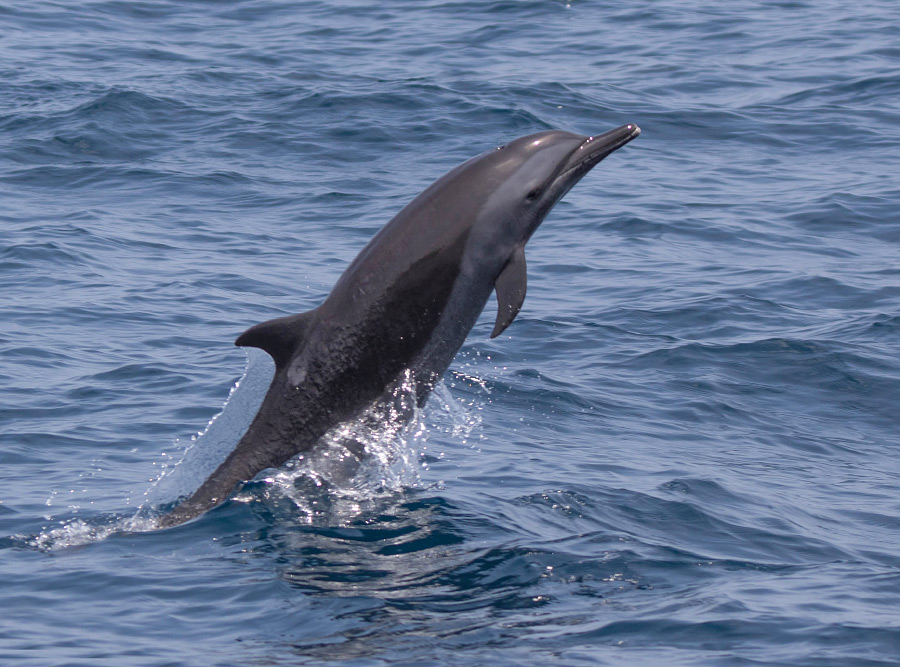
\includegraphics[width=0.45\textwidth]{dolphin}
\caption{வௌவால் மற்றும் டால்பின் --- மீயொலி மூலம் திசையறிதல்}
\end{figure}

% ==========================================================
\section{குறுக்கலைகள் (Transverse Waves)}
% ==========================================================

ஒலி அலையானது \textbf{நெட்டலைக்கு} ஒரு சிறந்த உதாரணமாகும். ஆனால்,
\textbf{குறுக்கலை} எனப்படும் மற்றொரு வகை அலையும் உள்ளது.

\begin{tcolorbox}[conceptbox]
\begin{description}
  \item[\textbf{நெட்டலை (Longitudinal Wave)}] துகள்கள் அலை பரவும் திசையிலேயே
        அதிர்வடைகின்றன. ஒலி ஒரு நெட்டலை.
  \item[\textbf{குறுக்கலை (Transverse Wave)}] துகள்கள் அலை பரவும் திசைக்குச்
        செங்குத்தாக மேலும் கீழும் அதிர்வடைகின்றன.
\end{description}
\textbf{உதாரணம்:} ஒரு குளத்தில் கல்லை எறியும்போது நீரின் மேற்பரப்பில் உருவாகும் அலைகள்.
ஒளி ஒரு குறுக்கலையாகும் --- ஆனால் ஒளி ஒரு இயந்திர அலை அல்ல.
\end{tcolorbox}

\bigskip\bigskip

\begin{center}
\small\textit{ஒலி --- எட்டாம் வகுப்பு அறிவியல் | TNSCERT | தமிழாக்கம் 2025--2026}
\end{center}

\end{document}
